\section{实验}
\label{sec:experiment}

这一章节将会利用上一章介绍的三种模版匹配方法在模版图像和场景图像上进行实验,并对其定位精度、定位效率进行展示和分析。

\twocolumn[{%
\renewcommand\twocolumn[1][]{#1}%
\noindent\begin{minipage}{\linewidth} 
 	\begin{center}
 	\vspace{0.3cm}
 	\captionsetup{font=small}
 	\begin{tabular}{@{}c@{}c@{}c@{}}
	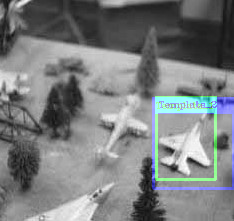
\includegraphics[width=0.33\linewidth]{correlation} &
 	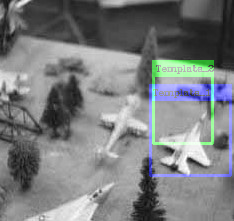
\includegraphics[width=0.33\linewidth]{hausdorff} &
    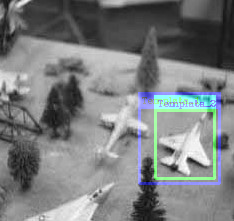
\includegraphics[width=0.33\linewidth]{distance_transform} \vspace{-1mm}\\
    {\small (a)} &  {\small (b)}  &  {\small (c)} \\
    \end{tabular}
	\captionof{figure}{\small 不同方法的模版匹配结果: (a) 相关匹配方法, (b) Hausdorff 距离匹配方法, and (c) 图像距离变换匹配方法}
	\label{fig:result}
	\end{center}
	\vspace{0.5cm}
\end{minipage}
}]

如图 \ref{fig:result} 所示,(a)、(b)、(c) 分别为相关匹配方法、Hausdorff 距离匹配方法和图像距离变换方法的匹配结果。可以看到,相关匹配方法和图像距离变换方法的定位精度优于 Hausdorff 距离匹配方法,尤其就第二幅模版图像而言。而对比两幅模版的定位精度时,显然可以看到对于相关匹配方法和图像距离变换方法,第二幅模版图像的定位精度优于第一幅模版图像,其原因在于第一幅模版图像与场景图像的相似内容有一定的尺寸、旋转偏差,从而导致第一幅模版图像的定位精度欠佳。但同样对于 Hausdorff 距离匹配方法,第一幅模版图像的定位精度却优于第二幅模版图像,这可能是由于边缘检测结果欠佳造成的,如设置了不合适的阈值,导致边缘点较少等。

\begin{figure}[!ht]
  \centering
  \begin{minipage}[b]{\linewidth} 
  \subfloat[]{
    \begin{minipage}[b]{0.3\linewidth} 
      \centering
      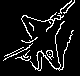
\includegraphics[width=\linewidth]{0template}\vspace{2pt}
      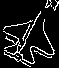
\includegraphics[width=\linewidth]{1template}
       \end{minipage}
  }
  \subfloat[]{
    \begin{minipage}[b]{0.67\linewidth} 
      \centering
      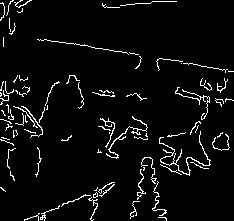
\includegraphics[width=\linewidth]{scene}
       \end{minipage}
  }
  \end{minipage}
  \vfill
  \caption{基于 Canny 算法提取的图像边缘:(a) 模版图像, (b) 场景图像.}
  \label{fig:edge}
\end{figure}


如图 \ref{fig:edge} 所示,为利用 Canny 算法提取的模版图像和场景图像的边缘。可以看到,第一幅模版图像的边缘较为连续,而第二幅模版图像的边缘在右上角有类似于“噪声”的点,这些“噪声点”会在一定程度上影响到 Hausdorff 距离的计算,进而影响到最后的定位结果。

\begin{table}[!htbp]
\caption{不同匹配方法的定位效率比较}
\centering
\label{tab:measurement}
\setlength{\tabcolsep}{0.2mm}{
\begin{tabular}{c|c|c|c}
\hline
& 相关匹配方法 & Hausdorff 距离匹配方法 & 图像距离变换方法\\
\hline
运行时间(秒) & 2.66 & 15.48 & 2.28\\
\hline
\end{tabular}
}
\end{table}

从定位效率来看,如表 \ref{tab:measurement} 所示,相关匹配方法和图像距离变换方法的定位效率远高于 Huasdorff 距离匹配方法,如图 \ref{fig:transform} 所示,图像距离变换的方法是预先计算出了图像矩阵中距离边缘点最近的切比雪夫距离,从而在匹配过程中只需要查找得到当前位置的距离,以此提高定位效率。出自之外,其定位精度相对于 Huasdorff 距离匹配方法也有所提升,可能是由于相对于 Huasdorff 距离,该方法鲁棒性更强。

\begin{figure}[!ht]
\centering
  \begin{minipage}[b]{\linewidth} 
  \subfloat[]{
    \begin{minipage}[b]{0.63\linewidth} 
      \centering
            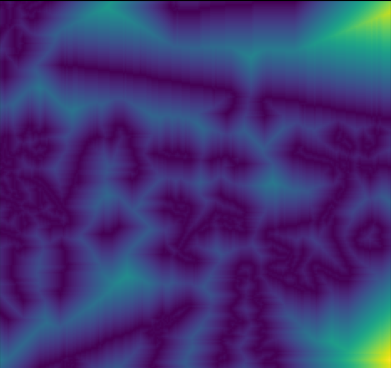
\includegraphics[width=\linewidth]{myplot}
       \end{minipage}
  }
  \subfloat[]{
    \begin{minipage}[b]{0.4\linewidth} 
      \centering
      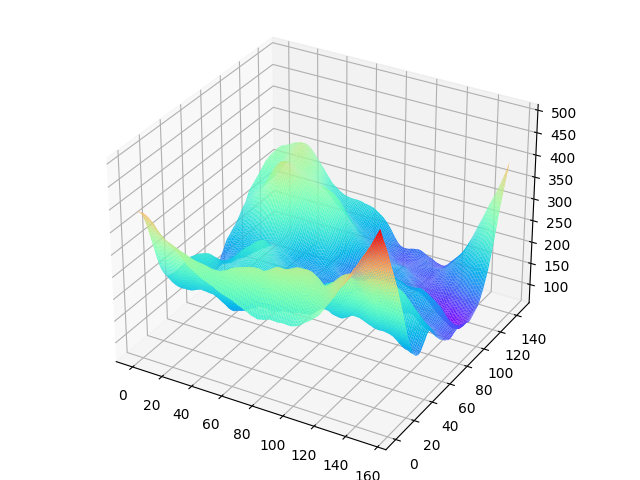
\includegraphics[width=\linewidth]{myplot1}\vspace{2pt}
      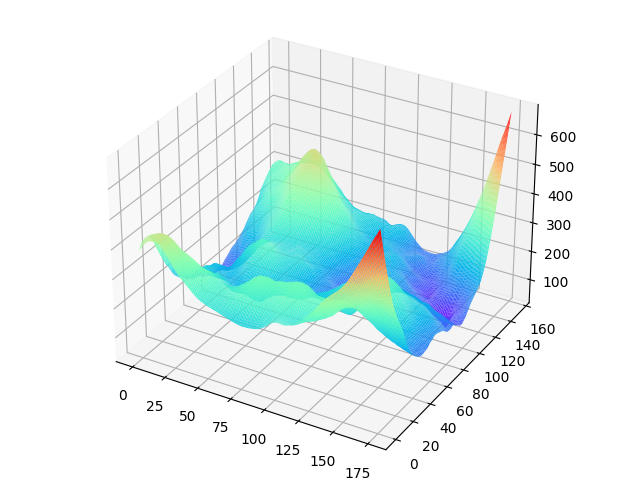
\includegraphics[width=\linewidth]{myplot2}
       \end{minipage}
  }
  \end{minipage}
  \vfill
  \caption{图像距离变换可视化结果:(a) 场景图像距离变换可视化, (b) 模版图像距离分布.}
	\label{fig:transform}
\end{figure}
